\documentclass{beamer}
\usepackage{amsmath,graphics}
\usepackage{amssymb}

\usetheme{default}
\usepackage{xcolor}

\definecolor{solarizedBase03}{HTML}{002B36}
\definecolor{solarizedBase02}{HTML}{073642}
\definecolor{solarizedBase01}{HTML}{586e75}
\definecolor{solarizedBase00}{HTML}{657b83}
\definecolor{solarizedBase0}{HTML}{839496}
\definecolor{solarizedBase1}{HTML}{93a1a1}
\definecolor{solarizedBase2}{HTML}{EEE8D5}
\definecolor{solarizedBase3}{HTML}{FDF6E3}
\definecolor{solarizedYellow}{HTML}{B58900}
\definecolor{solarizedOrange}{HTML}{CB4B16}
\definecolor{solarizedRed}{HTML}{DC322F}
\definecolor{solarizedMagenta}{HTML}{D33682}
\definecolor{solarizedViolet}{HTML}{6C71C4}
%\definecolor{solarizedBlue}{HTML}{268BD2}
\definecolor{solarizedBlue}{HTML}{134676}
\definecolor{solarizedCyan}{HTML}{2AA198}
\definecolor{solarizedGreen}{HTML}{859900}
\definecolor{myBlue}{HTML}{162DB0}%{261CA4}
\setbeamercolor*{item}{fg=myBlue}
\setbeamercolor{normal text}{fg=solarizedBase03, bg=solarizedBase3}
\setbeamercolor{alerted text}{fg=myBlue}
\setbeamercolor{example text}{fg=myBlue, bg=solarizedBase3}
\setbeamercolor*{frametitle}{fg=solarizedRed}
\setbeamercolor*{title}{fg=solarizedRed}
\setbeamercolor{block title}{fg=myBlue, bg=solarizedBase3}
\setbeameroption{hide notes}
\setbeamertemplate{note page}[plain]
\beamertemplatenavigationsymbolsempty
\usefonttheme{professionalfonts}
\usefonttheme{serif}

\usepackage{fourier}

\def\vec#1{\mathchoice{\mbox{\boldmath$\displaystyle#1$}}
{\mbox{\boldmath$\textstyle#1$}}
{\mbox{\boldmath$\scriptstyle#1$}}
{\mbox{\boldmath$\scriptscriptstyle#1$}}}
\definecolor{OwnGrey}{rgb}{0.560,0.000,0.000} % #999999
\definecolor{OwnBlue}{rgb}{0.121,0.398,0.711} % #1f64b0
\definecolor{red4}{rgb}{0.5,0,0}
\definecolor{blue4}{rgb}{0,0,0.5}
\definecolor{Blue}{rgb}{0,0,0.66}
\definecolor{LightBlue}{rgb}{0.9,0.9,1}
\definecolor{Green}{rgb}{0,0.5,0}
\definecolor{LightGreen}{rgb}{0.9,1,0.9}
\definecolor{Red}{rgb}{0.9,0,0}
\definecolor{LightRed}{rgb}{1,0.9,0.9}
\definecolor{White}{gray}{1}
\definecolor{Black}{gray}{0}
\definecolor{LightGray}{gray}{0.8}
\definecolor{Orange}{rgb}{0.1,0.2,1}
\setbeamerfont{sidebar right}{size=\scriptsize}
\setbeamercolor{sidebar right}{fg=Black}

\renewcommand{\emph}[1]{{\textcolor{solarizedRed}{\itshape #1}}}

\newcommand\tay{T}
\newcommand\dd{\mathrm d}
\newcommand\eul{\mathrm e}

\newcommand\cA{\mathcal A}
\newcommand\cB{\mathcal B}
\newcommand\cC{\mathcal C}
\newcommand\cD{\mathcal D}
\newcommand\cE{\mathcal E}
\newcommand\cF{\mathcal F}
\newcommand\cG{\mathcal G}
\newcommand\cH{\mathcal H}
\newcommand\cI{\mathcal I}
\newcommand\cJ{\mathcal J}
\newcommand\cK{\mathcal K}
\newcommand\cL{\mathcal L}
\newcommand\cM{\mathcal M}
\newcommand\cN{\mathcal N}
\newcommand\cO{\mathcal O}
\newcommand\cP{\mathcal P}
\newcommand\cQ{\mathcal Q}
\newcommand\cR{\mathcal R}
\newcommand\cS{\mathcal S}
\newcommand\cT{\mathcal T}
\newcommand\cU{\mathcal U}
\newcommand\cV{\mathcal V}
\newcommand\cW{\mathcal W}
\newcommand\cX{\mathcal X}
\newcommand\cY{\mathcal Y}
\newcommand\cZ{\mathcal Z}

\newcommand\fA{\mathfrak A}
\newcommand\fB{\mathfrak B}
\newcommand\fC{\mathfrak C}
\newcommand\fD{\mathfrak D}
\newcommand\fE{\mathfrak E}
\newcommand\fF{\mathfrak F}
\newcommand\fG{\mathfrak G}
\newcommand\fH{\mathfrak H}
\newcommand\fI{\mathfrak I}
\newcommand\fJ{\mathfrak J}
\newcommand\fK{\mathfrak K}
\newcommand\fL{\mathfrak L}
\newcommand\fM{\mathfrak M}
\newcommand\fN{\mathfrak N}
\newcommand\fO{\mathfrak O}
\newcommand\fP{\mathfrak P}
\newcommand\fQ{\mathfrak Q}
\newcommand\fR{\mathfrak R}
\newcommand\fS{\mathfrak S}
\newcommand\fT{\mathfrak T}
\newcommand\fU{\mathfrak U}
\newcommand\fV{\mathfrak V}
\newcommand\fW{\mathfrak W}
\newcommand\fX{\mathfrak X}
\newcommand\fY{\mathfrak Y}
\newcommand\fZ{\mathfrak Z}

\newcommand\fa{\mathfrak a}
\newcommand\fb{\mathfrak b}
\newcommand\fc{\mathfrak c}
\newcommand\fd{\mathfrak d}
\newcommand\fe{\mathfrak e}
\newcommand\ff{\mathfrak f}
\newcommand\fg{\mathfrak g}
\newcommand\fh{\mathfrak h}
%\newcommand\fi{\mathfrak i}
\newcommand\fj{\mathfrak j}
\newcommand\fk{\mathfrak k}
\newcommand\fl{\mathfrak l}
\newcommand\fm{\mathfrak m}
\newcommand\fn{\mathfrak n}
\newcommand\fo{\mathfrak o}
\newcommand\fp{\mathfrak p}
\newcommand\fq{\mathfrak q}
\newcommand\fr{\mathfrak r}
\newcommand\fs{\mathfrak s}
\newcommand\ft{\mathfrak t}
\newcommand\fu{\mathfrak u}
\newcommand\fv{\mathfrak v}
\newcommand\fw{\mathfrak w}
\newcommand\fx{\mathfrak x}
\newcommand\fy{\mathfrak y}
\newcommand\fz{\mathfrak z}

\newcommand\vA{\vec A}
\newcommand\vB{\vec B}
\newcommand\vC{\vec C}
\newcommand\vD{\vec D}
\newcommand\vE{\vec E}
\newcommand\vF{\vec F}
\newcommand\vG{\vec G}
\newcommand\vH{\vec H}
\newcommand\vI{\vec I}
\newcommand\vJ{\vec J}
\newcommand\vK{\vec K}
\newcommand\vL{\vec L}
\newcommand\vM{\vec M}
\newcommand\vN{\vec N}
\newcommand\vO{\vec O}
\newcommand\vP{\vec P}
\newcommand\vQ{\vec Q}
\newcommand\vR{\vec R}
\newcommand\vS{\vec S}
\newcommand\vT{\vec T}
\newcommand\vU{\vec U}
\newcommand\vV{\vec V}
\newcommand\vW{\vec W}
\newcommand\vX{\vec X}
\newcommand\vY{\vec Y}
\newcommand\vZ{\vec Z}

\newcommand\va{\vec a}
\newcommand\vb{\vec b}
\newcommand\vc{\vec c}
\newcommand\vd{\vec d}
\newcommand\ve{\vec e}
\newcommand\vf{\vec f}
\newcommand\vg{\vec g}
\newcommand\vh{\vec h}
\newcommand\vi{\vec i}
\newcommand\vj{\vec j}
\newcommand\vk{\vec k}
\newcommand\vl{\vec l}
\newcommand\vm{\vec m}
\newcommand\vn{\vec n}
\newcommand\vo{\vec o}
\newcommand\vp{\vec p}
\newcommand\vq{\vec q}
\newcommand\vr{\vec r}
\newcommand\vs{\vec s}
\newcommand\vt{\vec t}
\newcommand\vu{\vec u}
\newcommand\vv{\vec v}
\newcommand\vw{\vec w}
\newcommand\vx{\vec x}
\newcommand\vy{\vec y}
\newcommand\vz{\vec z}

\renewcommand\AA{\mathbb A}
\newcommand\NN{\mathbb N}
\newcommand\ZZ{\mathbb Z}
\newcommand\PP{\mathbb P}
\newcommand\QQ{\mathbb Q}
\newcommand\RR{\mathbb R}
\newcommand\RRpos{\mathbb R_{\geq0}}
\renewcommand\SS{\mathbb S}
\newcommand\CC{\mathbb C}

\newcommand{\ord}{\mathrm{ord}}
\newcommand{\id}{\mathrm{id}}
\newcommand{\pr}{\mathrm{P}}
\newcommand{\Vol}{\mathrm{vol}}
\newcommand\norm[1]{\left\|{#1}\right\|} 
\newcommand\sign{\mathrm{sign}}
\newcommand{\eps}{\varepsilon}
\newcommand{\abs}[1]{\left|#1\right|}
\newcommand\bc[1]{\left({#1}\right)} 
\newcommand\cbc[1]{\left\{{#1}\right\}} 
\newcommand\bcfr[2]{\bc{\frac{#1}{#2}}} 
\newcommand{\bck}[1]{\left\langle{#1}\right\rangle} 
\newcommand\brk[1]{\left\lbrack{#1}\right\rbrack} 
\newcommand\scal[2]{\bck{{#1},{#2}}} 
\newcommand{\vecone}{\mathbb{1}}
\newcommand{\tensor}{\otimes}
\newcommand{\diag}{\mathrm{diag}}
\newcommand{\ggt}{\mathrm{ggT}}
\newcommand{\kgv}{\mathrm{kgV}}
\newcommand{\trans}{\top}

\newcommand{\Karonski}{Karo\'nski}
\newcommand{\Erdos}{Erd\H{o}s}
\newcommand{\Renyi}{R\'enyi}
\newcommand{\Lovasz}{Lov\'asz}
\newcommand{\Juhasz}{Juh\'asz}
\newcommand{\Bollobas}{Bollob\'as}
\newcommand{\Furedi}{F\"uredi}
\newcommand{\Komlos}{Koml\'os}
\newcommand{\Luczak}{\L uczak}
\newcommand{\Kucera}{Ku\v{c}era}
\newcommand{\Szemeredi}{Szemer\'edi}

\renewcommand{\ae}{\"a}
\renewcommand{\oe}{\"o}
\newcommand{\ue}{\"u}
\newcommand{\Ae}{\"A}
\newcommand{\Oe}{\"O}
\newcommand{\Ue}{\"U}

\newcommand{\im}{\mathrm{im}}
\newcommand{\rrk}{\mathrm{zrg}}
\newcommand{\crk}{\mathrm{srg}}
\newcommand{\rk}{\mathrm{rg}}
\newcommand{\GL}{\mathrm{GL}}
\newcommand{\SL}{\mathrm{SL}}
\newcommand{\SO}{\mathrm{SO}}
\newcommand{\nul}{\mathrm{nul}}
\newcommand{\eig}{\mathrm{eig}}

\newcommand{\mytitle}{Das Newtonverfahren}

\title[Annuma]{\mytitle}
\author[Amin Coja-Oghlan]{Amin Coja-Oghlan}
\institute[Frankfurt]{JWGUFFM}
\date{}

\begin{document}

\frame[plain]{\titlepage}

\begin{frame}\frametitle{\mytitle}
	\begin{block}{Worum geht es?}
		\begin{itemize}
			\item Wir suchen numerische N\ae herungsl\oe sungen f\ue r Gleichungen der Form
				\begin{align*}
					f(x)=0.
				\end{align*}
			\item Dabei kann $f$ ein- oder mehrdimensional sein.
		\end{itemize}
	\end{block}
\end{frame}

\begin{frame}\frametitle{\mytitle}
	\begin{block}{Fixpunktprobleme}
		\begin{itemize}
			\item Anstatt die Gleichung $f(x)=0$ zu l\oe sen, versuchen wir uns an der Gleichung
				\begin{align*}
					x&=g(x)\qquad\mbox{wobei }g(x)=x+f(x).
				\end{align*}
			\item Eine Gleichung der Form $x=g(x)$ nennt man ein \alert{Fixpunktproblem}.
		\end{itemize}
	\end{block}
\end{frame}

\begin{frame}\frametitle{\mytitle}
	\begin{block}{Fixpunktprobleme}
		\begin{itemize}
			\item Eine naheliegende L\oe sungsstrategie ist, ausgehend von einem Startwert $x_0$ die Folge
				\begin{align*}
					x_{n+1}=g(x_n)&&(n\geq0)
				\end{align*}
				zu berechnen.
			\item Wenn die Folge konvergiert und $g$ stetig ist, dann gilt
				\begin{align*}
					\lim_{n\to\infty}x_n&=g\bc{\lim_{n\to\infty}x_n}.
				\end{align*}
			\item Das funktioniert im ein- wie auch im mehrdimensionalen Fall.
		\end{itemize}
	\end{block}
\end{frame}

\begin{frame}\frametitle{\mytitle}
	\begin{block}{Definition}
		\begin{itemize}
			\item Sei $I=[a,b]\subset\RR$ mit $a<b$ ein Intervall. 
			\item Eine Funktion $g:I\to I$ hei\ss t eine \emph{Kontraktion}, falls es eine Zahl $\eps>0$ gibt, so da\ss
				\begin{align*}
					\abs{g(x)-g(y)}<\exp(-\eps)|x-y|\qquad\mbox{f\ue r alle }x,y\in I.
				\end{align*}
		\end{itemize}
	\end{block}
\end{frame}

\begin{frame}\frametitle{\mytitle}
	\begin{block}{Proposition}
		\begin{itemize}
			\item Angenommen $g:I\to I$ ist stetig und auf $I^\circ$ differenzierbar.
			\item Angenommen ferner es gibt eine Zahl $\eps>0$, so da\ss
				\begin{align*}
					|g'(x)|<\exp(-\eps)&&\mbox{f\ue r alle }x\in I^\circ.
				\end{align*}
			\item Dann ist $g$ eine Kontraktion.
		\end{itemize}
	\end{block}
\end{frame}

\begin{frame}\frametitle{\mytitle}
	\begin{block}{Beispiel}
		\begin{itemize}
			\item Die Funktion $g:[0,1/3]\to[0,1/3]$, $x\mapsto x^2$ ist eine Kontraktion.
			\item Denn
				\begin{align*}
					g'(x)=2x
				\end{align*}
				ist betragsm\ae ssig $\leq\frac{2}{3}$ auf dem gesamten Intervall.
		\end{itemize}
	\end{block}
\end{frame}

\begin{frame}\frametitle{\mytitle}
	\begin{block}{Fixpunktsatz (eindimensional)}
		\begin{itemize}
			\item Wenn $g:I\to I$ eine Kontraktion ist, dann besitzt $g$ einen eindeutigen Fixpunkt in $I$.
			\item D.h.\ es gibt genau eine Zahl $x^*\in I$ mit $g(x^*)=x^*$.
			\item F\ue r jede Zahl $x_0\in I$ gilt
				\begin{align*}
					x^*=\lim_{n\to\infty}x_n\quad\mbox{mit}\quad x_{n+1}=g(x_n)\mbox{ f\ue r }n\geq0.
				\end{align*}
			\item {\itshape Die Konvergenz erfolgt `schnell'.}
		\end{itemize}
	\end{block}
\end{frame}

\begin{frame}\frametitle{\mytitle}
	\hfill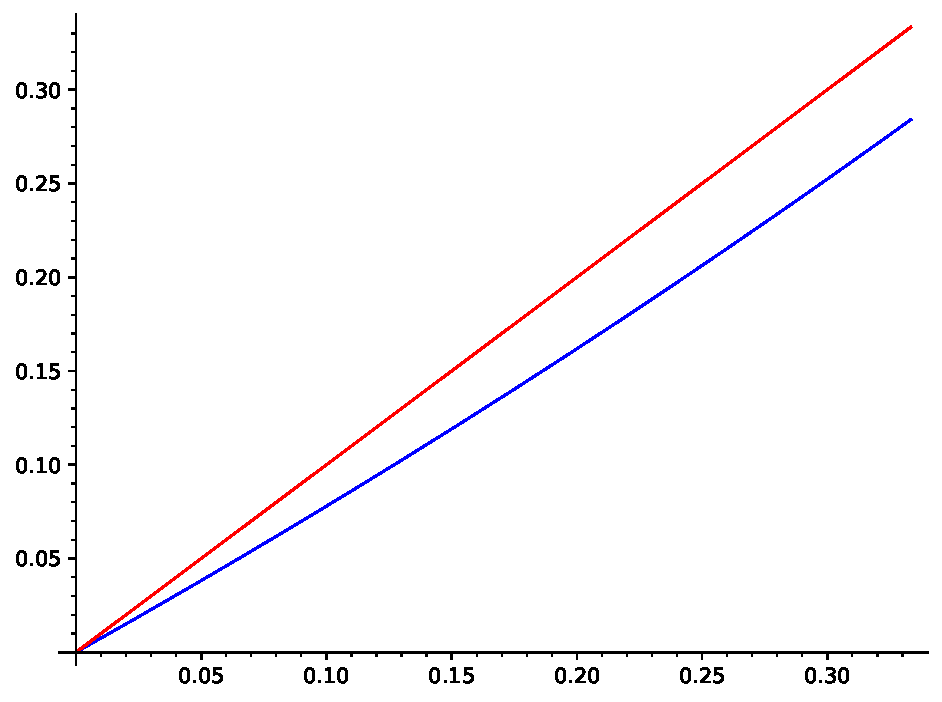
\includegraphics[height=30mm]{pics/plot_fix.pdf}
	\begin{block}{Beispiel}
		\begin{itemize}
			\item Sei $g:[0,1/3]\to[0,1/3]$ die Funktion $g(x)=\exp(3x/4)-1$.
			\item Die Ableitung ist
				\begin{align*}
					g'(x)=\frac{3}{4}\exp(3x/4)\in(0,0.99)
				\end{align*}
			\item Daher ist $g$ eine Kontraktion; der Fixpunkt ist $x^*=0$.
		\end{itemize}
	\end{block}
\end{frame}

\begin{frame}\frametitle{\mytitle}
	\begin{block}{Newtonverfahren (eindimensional)}
		\begin{itemize}
			\item Wir nehmen an, da\ss\ $f$ differenzierbar ist.
			\item Das Ziel ist, eine Nullstelle $f(x)=0$ zu berechnen.
			\item Dazu f\ue hren wir, ausgehend von einem Startwert, die Iteration
				\begin{align*}
					x_{n+1}&=x_n-\frac{f(x_n)}{f'(x_n)}
				\end{align*}
				durch, sofern $f'(x_n)\neq0$.
			\item Wenn $f,f'$ stetig sind und $f'(x)\neq0$ und
				\begin{align*}
					x^*=\lim_{n\to\infty}x_n
				\end{align*}
				existiert, dann ist $x^*$ eine Nullstelle von $f$.
		\end{itemize}
	\end{block}
\end{frame}

\begin{frame}\frametitle{\mytitle}
	\begin{block}{Beispiel}
		\begin{itemize}
			\item Wir suchen eine Nullstelle von $f(x)=x^2-2$.
			\item Die Iterationsformel lautet
				\begin{align*}
					x_{n+1}=x_n-\frac{f(x_n)}{f'(x_n)}=x_n-\frac{x_n^2-2}{2x_n}=\frac{x_n^2+2}{2x_n}
				\end{align*}
			\item Als Startwert w\ae hlen wir $x_0=1.4$.
			\item Die ersten Folgenglieder lauten
				\begin{align*}
					x_1&=1.414285714\cdots\\
					x_2&=1.414213564\cdots
				\end{align*}
			\item Die korrekte L\oe sung ist $x^*=\sqrt2 =1.414213562\cdots$.
		\end{itemize}
	\end{block}
\end{frame}

\begin{frame}\frametitle{\mytitle}
	\begin{block}{Satz}
		\begin{itemize}
			\item Angenommen $f(x)$ hat eine Nullstelle $\alpha$ und $f$ ist stetig differenzierbar.
			\item Angenommen ferner $f'(\alpha)\neq0$.
			\item Dann gibt es ein $\eps>0$, so da\ss\ das Newtonverfahren f\ue r alle Startwerte $x_0$ mit $|x_0-\alpha|<\eps$ gegen
				\begin{align*}
				x^*=\alpha
				\end{align*}
				konvergiert.
		\end{itemize}
	\end{block}
\end{frame}

\begin{frame}\frametitle{\mytitle}
	\begin{block}{Fixpunktprobleme (mehrdimensional)}
		\begin{itemize}
			\item Eine Menge $U\subset\RR^n$ ist \emph{abgeschlossen}, wenn f\ue r jede konvergente Folge $(a_n)_n$ mit $a_n\in U$ gilt, da\ss\ $$\lim_{n\to\infty}a_n\in U.$$
			\item Sei $U\subset\RR^n$ eine abgeschlossene Menge und sei
				$$f:U\to U$$
				eine Funktion.
			\item Ein \emph{Fixpunkt} ist ein Punkt $x\in U$ mit $f(x)=x$.
			\item Die Funktion $f$ ist eine \emph{Kontraktion}, falls es ein $\eps>0$ mit
				\begin{align*}
					\|f(x)-f(y)|\leq\exp(-\eps)\|x-y\|&&(x,y\in U)
				\end{align*}
				gibt.
		\end{itemize}
	\end{block}
\end{frame}

\begin{frame}\frametitle{\mytitle}
	\begin{block}{Fixpunktsatz (mehrdimensional)}
		\begin{itemize}
			\item Sei $U\subset\RR^n$ abgeschlossen.
			\item Sei $f:U\to U$ eine Kontraktion.
			\item Dann besitzt $f$ einen eindeutigen Fixpunkt in $U$.
			\item F\ue r jedes $x_0\in U$ konvergiert die Folge $(x_n)_n$ mit
				\begin{align*}
					x_{n+1}=f(x_n)
				\end{align*}
				gegen diesen Fixpunkt.
		\end{itemize}
	\end{block}
\end{frame}

\begin{frame}\frametitle{\mytitle}
	\begin{block}{Definition}
			F\ue r eine Funktion $f(x)$ mit $x,f(x)\in\RR^n$, deren partielle Ableitungen existieren, definieren wir die \emph{Jacobimatrix}
				\begin{align*}
					Df(x)&=\bc{\frac{\partial f_i}{\partial x_j}}_{i,j=1,\ldots,n}.
				\end{align*}
	\end{block}
\end{frame}

\begin{frame}\frametitle{\mytitle}
	\begin{block}{Definition}
		Eine Menge $U\subset\RR^n$ ist \emph{konvex}, falls f\ue r alle $u,v\in U$ und alle $\alpha\in[0,1]$ gilt
		\begin{align*}
			\alpha u+(1-\alpha)v\in U.
		\end{align*}
		{\itshape Intuition: f\ue r alle $u,v\in U$ liegt auch immer die ganze Strecke zwischen $u$ und $v$ in $U$.}
	\end{block}
\end{frame}

\begin{frame}\frametitle{\mytitle}
	\begin{block}{Proposition}
		\begin{itemize}
		\item Angenommen $U\subset\RR^n$ ist konvex.
		\item Angenommen $f:U\to\RR^n$ hat stetige partielle Ableitungen
			\begin{align*}
			\frac{\partial f_i}{\partial x_j}.
			\end{align*}
		\item Angenommen ferner es existiert ein $\eps>0$, so da\ss
			\begin{align*}
				\|Df(x)\|<\exp(-\eps)&&\mbox{f\ue r alle }x\in U.
			\end{align*}
		\item Dann ist $f$ eine Kontraktion.
		\end{itemize}
	\end{block}
\end{frame}

\begin{frame}\frametitle{\mytitle}
	\begin{block}{Beispiel}
		\begin{itemize}
			\item Sei $f\binom xy=\binom{(x-y)^2}{(x+y)^2}$ und $D=[-0.1,0.1]^2$.
			\item Die Menge $D$ ist konvex und die partiellen Ableitungen sind
				\begin{align*}
					\frac{\partial f_1}{\partial x}&=\frac{\partial(x-y)^2}{\partial x}=2x-2y\\
					\frac{\partial f_1}{\partial y}&=\frac{\partial(x-y)^2}{\partial y}=-2x+2y\\
					\frac{\partial f_2}{\partial x}&=\frac{\partial(x-y)^2}{\partial x}=2x+2y\\
					\frac{\partial f_2}{\partial y}&=\frac{\partial(x-y)^2}{\partial y}=2x+2y\\
				\end{align*}
		\end{itemize}
	\end{block}
\end{frame}

\begin{frame}\frametitle{\mytitle}
	\begin{block}{Beispiel (fortgesetzt)}
		\begin{itemize}
			\item Die Jacobimatrix lautet also
				\begin{align*}
					Df(x)&=\begin{pmatrix}
						2(x-y)&2(y-x)\\2(x+y)&2(x+y)
					\end{pmatrix}
				\end{align*}
			\item Die Matrixnorm ist beschr\ae nkt durch
				\begin{align*}
					\|Df(x)\|&\leq\sqrt{2(2(x-y))^2+2(2(x+y))^2}=2^{3/2}\sqrt{(x-y)^2+(x+y)^2}\\
							 &=2^{3/2}\sqrt{x^2-2xy+y^2+x^2+2xy+y^2}=4\sqrt{x^2+y^2}<1.
				\end{align*}
			\item Also ist $f$ eine Kontraktion; der Fixpunkt ist $\binom xy=\binom 00$.
		\end{itemize}
	\end{block}
\end{frame}

\begin{frame}\frametitle{\mytitle}
	\begin{block}{Newtonverfahren (mehrdimensional)}
		\begin{itemize}
			\item Sei $f:\RR^n\to\RR^n$ eine Funktion mit stetigen partiellen Ableitungen.
			\item Die Jacobimatrix $Df(x)$ sei invertierbar.
			\item Ausgehend von einem Startpunkt $x_0$ definiere
				\begin{align*}
					x_{n+1}&=x_n-Df(x_n)^{-1}f(x_n).
				\end{align*}
			\item Anstatt die inverse Matrix zu berechnen, kann man $x_{n+1}$ als L\oe sung des linearen Gleichungssystems
				\begin{align*}
					Df(x_n)(x_{n+1}-x_n)&=-f(x_n)
				\end{align*}
				bestimmen.
		\end{itemize}
	\end{block}
\end{frame}

\begin{frame}\frametitle{\mytitle}
	\begin{block}{Beispiel}
		\begin{itemize}
			\item Sei $f:\RR^2\to\RR^2$ die Funktion $\binom xy\mapsto\binom{\cos(x)}{\sin(y)}-\frac{1/\sqrt 2}{1/\sqrt 2}$.
			\item Die partiellen Ableitungen unserer Funktion sind
				\begin{align*}
					\frac{\partial\cos x}{\partial x}&=-\sin x&\frac{\partial\cos x}{\partial y}&=0\\
					\frac{\partial\sin y}{\partial x}&=0&\frac{\partial\sin y}{\partial y}&=\cos y
				\end{align*}
			\item Wir erhalten die Jacobimatrix
				\begin{align*}
					Df(x)&=\begin{pmatrix} -\sin x&0\\0&\cos y \end{pmatrix}
				\end{align*}
		\end{itemize}
	\end{block}
\end{frame}

\begin{frame}\frametitle{\mytitle}
	\begin{block}{Beispiel}
		\begin{itemize}
			\item Die inverse Matrix lautet
				\begin{align*}
					Df(x)^{-1}&=\begin{pmatrix} -1/\sin x&0\\0&1/\cos y \end{pmatrix}
				\end{align*}
			\item Ausgehend von $x_0=y_0=0.75$ erhalten wir also
				\begin{align*}
					x_1&=x_0-Df(x_0)^{-1}f(x_0)\approx\binom{0.78606}{0.78481}\\
					x_2&=x_1-Df(x_1)^{-1}f(x_1)\approx\binom{0.78540}{0.78540}
				\end{align*}
			\item Die exakte L\oe sung lautet $\binom{\pi/4}{\pi/4}\approx\binom{0.78540}{0.78540}.$
		\end{itemize}
	\end{block}
\end{frame}

\begin{frame}\frametitle{\mytitle}
	\begin{block}{Zusammenfassung}
		\begin{itemize}
			\item Das Newtonverfahren ist ein numerisches Verfahren zum L\oe sen nichtlinearer Gleichungen.
			\item Die mehrdimensionale Version des Verfahrens dient zum L\oe sen nichtlinearer Gleichungssysteme.
			\item Das Newtonverfahren beruht auf einer Fixpunktberechnung.
		\end{itemize}
	\end{block}
\end{frame}











\end{document}
